\documentclass{standalone}
\usepackage{tikz}
\usetikzlibrary{calc,fadings,decorations.pathreplacing, intersections}
\usepackage{verbatim}
\usetikzlibrary{intersections}
\newcommand\pgfmathsinandcos[3]{%
  \pgfmathsetmacro#1{sin(#3)}%
  \pgfmathsetmacro#2{cos(#3)}%
}
\newcommand\LongitudePlane[3][current plane]{%
  \pgfmathsinandcos\sinEl\cosEl{#2} % elevation
  \pgfmathsinandcos\sint\cost{#3} % azimuth
  \tikzset{#1/.style={cm={\cost,\sint*\sinEl,0,\cosEl,(0,0)}}}
}

\newcommand\LatitudePlane[3][current plane]{%
  \pgfmathsinandcos\sinEl\cosEl{#2} % elevation
  \pgfmathsinandcos\sint\cost{#3} % latitude
  \pgfmathsetmacro\yshift{\cosEl*\sint}
  \tikzset{#1/.style={cm={\cost,0,0,\cost*\sinEl,(0,\yshift)}}} %
}

\newcommand\shiftLatitudePlane[3][current plane]{%
  \pgfmathsinandcos\sinEl\cosEl{#2} % elevation
  \pgfmathsinandcos\sint\cost{#3} % latitude
  \pgfmathsetmacro\yshift{\cosEl*\sint}
  \tikzset{#1/.style={cm={\cost,0,0,\cost*\sinEl,(0,0.25+\yshift)}}} %
}

\newcommand\NewLatitudePlane[4][current plane]{%
  \pgfmathsinandcos\sinEl\cosEl{#3} % elevation
  \pgfmathsinandcos\sint\cost{#4} % latitude
  \pgfmathsetmacro\yshift{#2*\cosEl*\sint}
  \tikzset{#1/.style={cm={\cost,0,0,\cost*\sinEl,(0,\yshift)}}} %
}
\newcommand\DrawLongitudeCircle[2][1]{
  \LongitudePlane{\angEl}{#2}
  \tikzset{current plane/.prefix style={scale=#1}}
   % angle of "visibility"
  \pgfmathsetmacro\angVis{atan(sin(#2)*cos(\angEl)/sin(\angEl))} %
  \draw[current plane] (\angVis:1) arc (\angVis:\angVis+180:1);
  \draw[current plane,dashed] (\angVis-180:1) arc (\angVis-180:\angVis:1);
}
\newcommand\DrawLatitudeCircle[2][1]{
  \LatitudePlane{\angEl}{#2}
  \tikzset{current plane/.prefix style={scale=#1}}
  \pgfmathsetmacro\sinVis{sin(#2)/cos(#2)*sin(\angEl)/cos(\angEl)}
  % angle of "visibility"
  \pgfmathsetmacro\angVis{asin(min(1,max(\sinVis,-1)))}
  \draw[current plane] (\angVis:1) arc (\angVis:-\angVis-180:1);
  \draw[current plane,dashed] (180-\angVis:1) arc (180-\angVis:\angVis:1);
}
\tikzset{%
    add/.style args={#1 and #2}{
        to path={%
 ($(\tikztostart)!-#1!(\tikztotarget)$)--($(\tikztotarget)!-#2!(\tikztostart)$)%
  \tikztonodes},add/.default={.2 and .2}}
}  
\tikzset{%
  >=latex, % option for nice arrows
  inner sep=0pt,%
  outer sep=2pt,%
  mark coordinate/.style={inner sep=0pt,outer sep=0pt,minimum size=3pt,
    fill=black,circle}%
}

\begin{document}



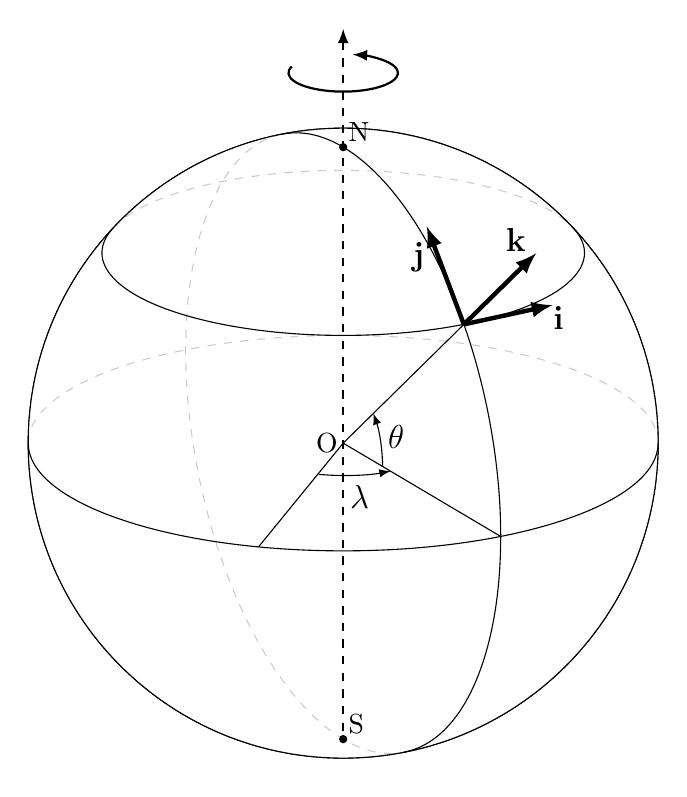
\begin{tikzpicture} % "THE GLOBE" showcase
\def\R{4 } % sphere radius
\def\angEl{20} % elevation angle
\def\angAz{-20} % azimuth angle

\def\latP{ 40} % Latitude of point P
\def\lonP{-60} % Longitude of point P

\def\deltaLat{10}
\def\deltaLon{10}

\def\constOpacity{0}
\def\BackOpacity{0.2}
%
% Draw the sphere
%
\filldraw[ball color=white] (0,0) circle (\R);
\filldraw[fill=white] (0,0) circle (\R);

% Draw the Equatorial Plane
    \LatitudePlane{\angEl}{0}
    \tikzset{current plane/.prefix style={scale=\R}}
    \pgfmathsetmacro\sinVis{sin(\latP)/cos(\latP)*sin(\angEl)/cos(\angEl)}
    % angle of "visibility"
    \pgfmathsetmacro\angVis{asin(min(1,max(\sinVis,-1)))}
    \draw[current plane, name path = equator] (0:1) arc (0:-180:1);
    \draw[current plane,dashed, opacity=\BackOpacity] (180:1) arc (180:0:1);
    \draw[current plane,->] (-105:0.3) arc (-105:\lonP:0.3);
%
% DEFINE THE PLANE FOR THE MAIN PARALLEL
%
  \LatitudePlane{\angEl}{\latP}
  \tikzset{current plane/.prefix style={scale=\R}}
  \pgfmathsetmacro\sinVis{sin(\latP)/cos(\latP)*sin(\angEl)/cos(\angEl)}
  % angle of "visibility"
  \pgfmathsetmacro\angVis{asin(min(1,max(\sinVis,-1)))}
  \draw[current plane, name path = parallel] (\angVis:1) arc (\angVis:-\angVis-180:1);
  \draw[current plane,dashed, opacity=\BackOpacity] (180-\angVis:1) arc (180-\angVis:\angVis:1);
%
% DEFINE THE PLANE FOR THE DELTA PARALLEL
%
  \LatitudePlane{\angEl}{\latP + \deltaLat/2}
  \tikzset{current plane/.prefix style={scale=\R}}
  \pgfmathsetmacro\sinVis{sin(\latP)/cos(\latP)*sin(\angEl)/cos(\angEl)}
  % angle of "visibility"
  \pgfmathsetmacro\angVis{asin(min(1,max(\sinVis,-1)))}
  \draw[current plane,blue, opacity = \constOpacity,  name path = deltaParallel] (\angVis:1) arc (\angVis:-\angVis-180:1);
%
% DEFINE THE PLANE FOR THE MAIN MERIDIAN
%
  \LongitudePlane{\angEl}{\lonP }
  \tikzset{current plane/.prefix style={scale=\R}}
   % angle of "visibility"
  \pgfmathsetmacro\angVis{atan(sin(\lonP)*cos(\angEl)/sin(\angEl))} %
  \draw [current plane, name path = meridian] (\angVis:1) arc (\angVis:\angVis+180:1);
  \draw[current plane,dashed, opacity=\BackOpacity] (\angVis-180:1) arc (\angVis-180:\angVis:1);
%
% DEFINE THE PLANE FOR THE DELTA MERIDIAN
%
  \LongitudePlane{\angEl}{\lonP+ \deltaLon/2}
  \tikzset{current plane/.prefix style={scale=\R}}
   % angle of "visibility"
  \pgfmathsetmacro\angVis{atan(sin(\lonP)*cos(\angEl)/sin(\angEl))} %
  \draw [current plane, blue, opacity = \constOpacity, name path = deltaMeridian] (\angVis:1) arc (\angVis:\angVis+180:1);

  \LongitudePlane{\angEl}{110}
  \tikzset{current plane/.prefix style={scale=\R}}
   % angle of "visibility"
  \pgfmathsetmacro\angVis{atan(sin(\lonP)*cos(\angEl)/sin(\angEl))} %
  \draw [current plane, opacity = \constOpacity, name path = meridian0] (\angVis:1) arc (\angVis:\angVis+180:1);
%\draw[current plane,->] (-180:0.3) arc (-180:-180-\latP:0.3);  



   % Intersections
   \path [name intersections={of=deltaParallel and meridian, by=North}];
   \path [name intersections={of=deltaMeridian and parallel, by=East}];
   \path [name intersections={of=meridian and parallel, by=centre}];
   \path [name intersections={of=meridian and equator, by=lat0}];
   \path [name intersections={of=meridian0 and equator, by=lon0}];
   
   \draw (0,0) -- (centre) ; % zero-lambda
   \draw (0,0) -- (lat0) ; % zero-lambda
   \draw (0,0) -- (lon0) ; % zero-lambda
   
   \draw[ opacity = \constOpacity ] (0,0) -- (East) ; % zero-lambda
   \draw[ opacity = \constOpacity ]  (0,0) -- (centre); % zero-lambda
   \draw[ opacity = \constOpacity ]  (0,0) -- (North); %      lambda

\draw [add= 0 and \R, black, ultra thick, ->] (centre) to (East);
\draw [add= 0 and 3*\R/4, black, ultra thick, ->] (centre) to (North);
\draw [add= -1 and .6, black, ultra thick, ->] (0,0) to (centre);

\pgfmathsetmacro\H{\R*cos(\angEl)}                    % distance to north pole
\coordinate (O) at (0,0);
\draw[left]                       node at (0,0)  {O}; % Origin label
\draw[right, anchor = south west] node at (0, \H){N}; % North Label
\draw[right, anchor = south west] node at (0,-\H){S}; % South Label
\coordinate[mark coordinate] (N) at (0, \H);
\coordinate[mark coordinate] (S) at (0,-\H);
\draw[add= 0.2 and 0, thick, dashed, black, <-] (N) to (S);
\node[circle,draw,black,scale=0.3] at (0,0) {};




\LongitudePlane[angle]{\angEl}{\lonP};
\draw[angle,->] (0:1) arc (0:\latP:1);

  \LatitudePlane{\angEl}{0}
  \tikzset{current plane/.prefix style={scale=\R}}
  \pgfmathsetmacro\sinVis{sin(\latP)/cos(\latP)*sin(\angEl)/cos(\angEl)}
  % angle of "visibility"
  \pgfmathsetmacro\angVis{asin(min(1,max(\sinVis,-1)))}
%\draw[current plane,-] (-105:0.3) arc (-105:\lonP:0.3);


  \shiftLatitudePlane{\angEl}{80}
  \tikzset{current plane/.prefix style={scale=\R}}
  \pgfmathsetmacro\sinVis{sin(\latP)/cos(\latP)*sin(\angEl)/cos(\angEl)}
  % angle of "visibility"
  \pgfmathsetmacro\angVis{asin(min(1,max(\sinVis,-1)))}
  \draw[current plane, thick, ->] (-200:1) arc (-200:80:1);

\draw[right, anchor = south east ] node at (1.1,2.1) {\large$\mathbf{j}$};
\draw[right, anchor = north west ] node at (2.6,1.8) {\large$\mathbf{i}$};
\draw[right, anchor = north west ] node at (2  ,2.8) {\large$\mathbf{k}$};



\draw[right, anchor = south east ] node at (0.4,-0.9) {\large$\lambda$};
\draw[right, anchor = north west ] node at (0.5,0.3) {\large$\theta$};


\end{tikzpicture}

\end{document}